\section{Interfaz de Usuario}

La interacción del operador con el sistema se realiza a través de dos canales: un dashboard y bot de Telegram. Ambas interfaces operan sobre flujos de datos asincrónicos.

\subsection{Dashboard}

El tablero de control web funciona como una aplicación de página única, estructurada sobre primitivas de HTML5, JavaScript moderno (ES6+) y CSS nativo sin dependencias pesadas.

La representación gráfica del terreno y de las unidades ganaderas se ejecuta mediante la biblioteca de \textit{Leaflet.js}. Al iniciar la sesión, el cliente realiza una petición HTTP inicial hacia el endpoint \texttt{GET /api/fence/current} para obtenerj el cerco activo de la base de datos y trazar el polígono delimitador sobre la capa del mapa.

De manera paralela, la aplicación establece un canal de comunicación dúplex persistente mediante \textit{WebSocket} contra el motor Node-RED. Cada vez que el Gateway ingesta un nuevo paquete de telemetría por radio LoRa, el servidor retransmite el evento \texttt{update\_location} a los clientes web conectados. La lógica del frontend actualiza de inmediato las coordenadas del marcador correspondiente al animal, la información del enlace, el nivel de voltaje de la batería y la última marca de tiempo de sincronización.

Para permitir un ajuste de los límites del perímetro virtual sobre el terreno, la interfaz incorpora un panel lateral interactivo de vértices que habilita la modificación de la geocerca mediante eventos de teclado.

Al finalizar el ajuste, el operador acciona el comando de guardado, lo que desencadena la emisión de una petición \texttt{POST /api/update-fence}. El servidor recibe la nueva geometría, recalcula la caja (\textit{Bounding Box}) y actualiza en milisegundos las reglas de validación en todos los nodos de monitoreo activos, tal como se ilustra en la Figura~\ref{fig:dashboard_web}.

\begin{figure}[H]
    \centering
    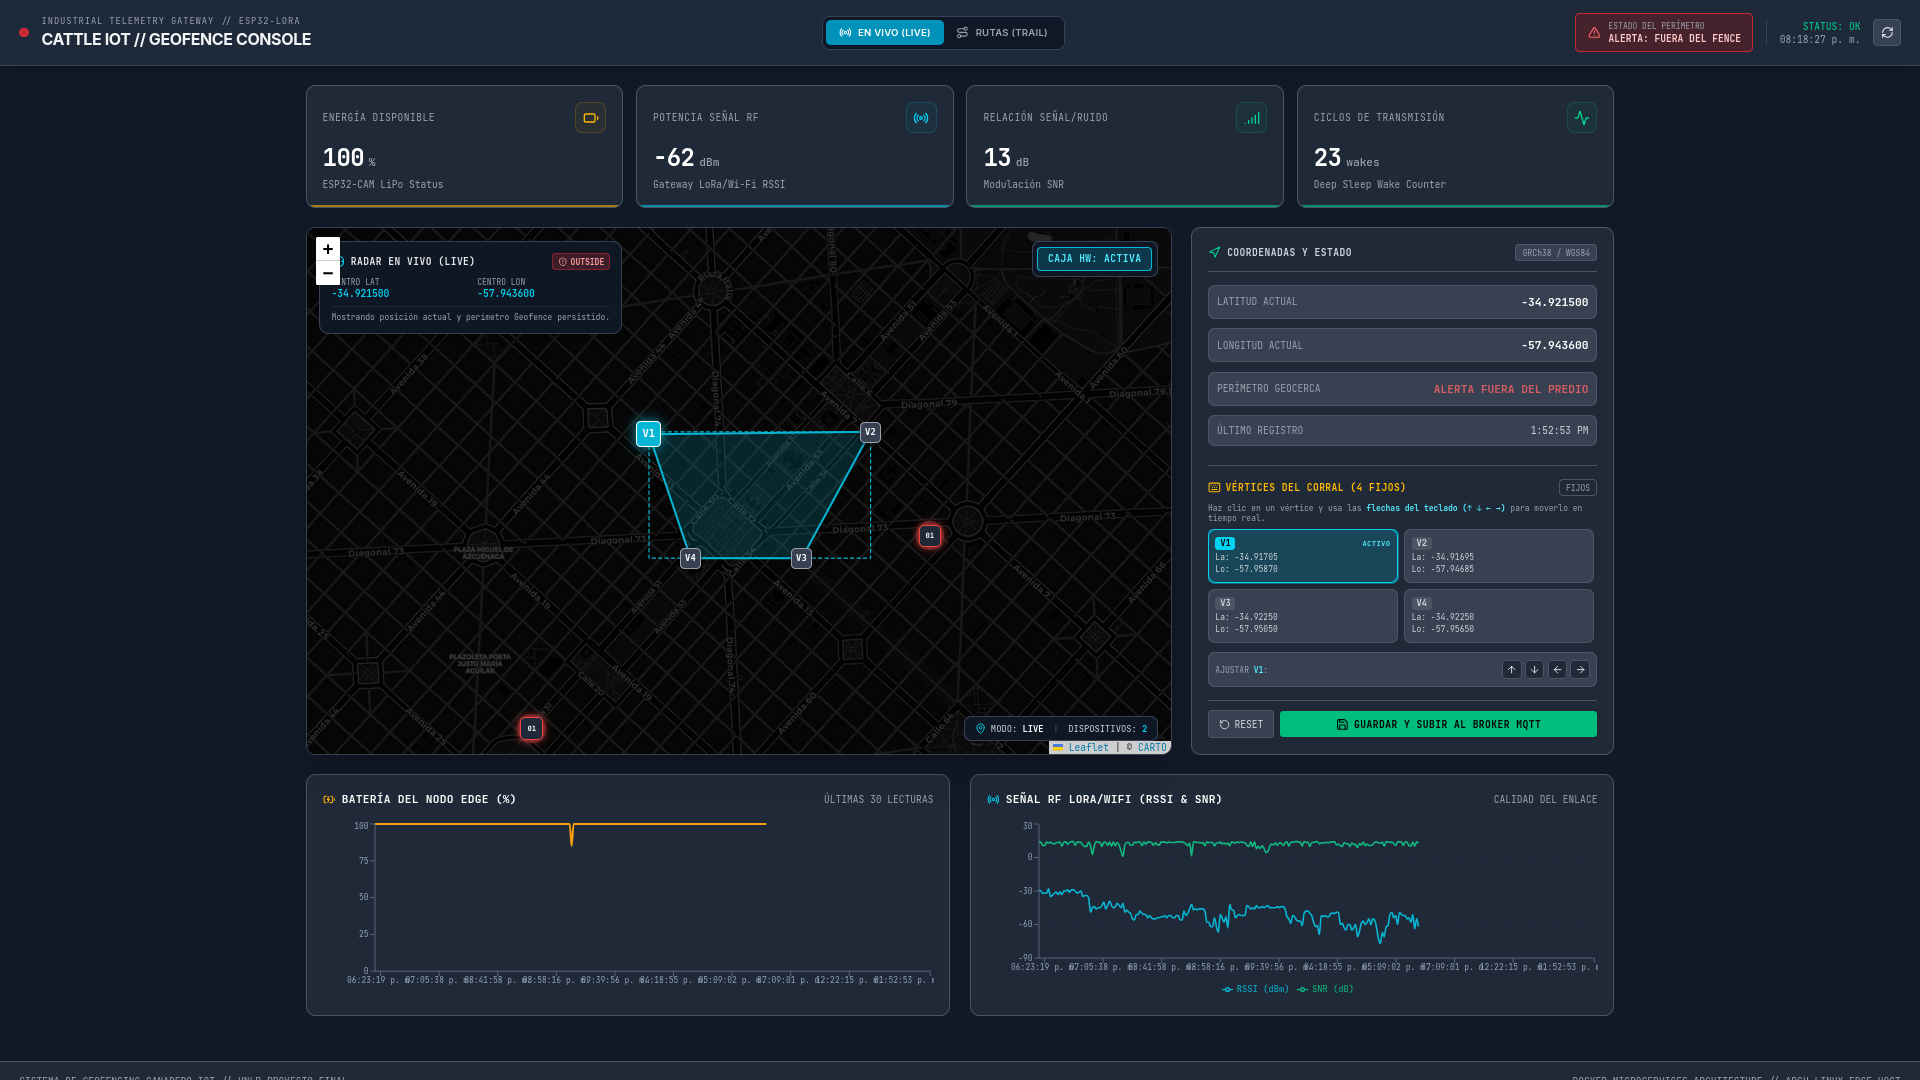
\includegraphics[width=0.98\textwidth]{secciones/image.png}
    \caption{Captura de pantalla del Dashboard.}
    \label{fig:dashboard_web}
\end{figure}

\subsection{Bot de Telegram}

La supervisión remota requiere un mecanismo de notificación push que no dependa de mantener un navegador web abierto continuamente. Para ello, el backend integra un bot de Telegram gestionado por la biblioteca \texttt{node-telegram-bot-api} dentro del entorno de Node-RED.

Cuando el algoritmo determina que la posición censada de un animal sale del cerco (\texttt{inside === false}), el módulo de notificaciones consulta en InfluxDB las últimas coordenadas reportadas del identificador del collar y estructura un mensaje de advertencia hacia los operadores.

El bot de Telegram opera como terminal de comandos remota, permitiendo al administrador del sistema intervenir de manera directa sobre los actuadores físicos del collar sin necesidad de acceder a la consola de servidor o al tablero web.

